% Author: Izaak Neutelings (September 2020)
% Inspiration: https://tex.stackexchange.com/questions/25531/adding-underbrace-in-tikz
\documentclass[border=3pt,tikz]{standalone}
\usepackage{physics}
\usepackage{ifthen}
\usepackage{tikz}
\usepackage[outline]{contour} % glow around text
\usetikzlibrary{calc} % for pic
\usetikzlibrary{angles,quotes} % for pic
\usetikzlibrary{patterns,snakes}
\tikzset{>=latex} % for LaTeX arrow head
\contourlength{1.2pt}

\colorlet{myred}{red!65!black}
\tikzstyle{ground}=[preaction={fill,top color=black!10,bottom color=black!5,shading angle=20},
                    fill,pattern=north east lines,draw=none,minimum width=0.3,minimum height=0.6]
\tikzstyle{mass}=[line width=0.6,red!30!black,fill=red!40!black!10,rounded corners=1,
                  top color=red!40!black!20,bottom color=red!40!black!10,shading angle=20]
\tikzstyle{rope}=[brown!70!black,line width=1.2,line cap=round] %very thick

% FORCES SWITCH
\tikzstyle{force}=[->,myred,thick,line cap=round]
\tikzstyle{Fproj}=[force,myred!40]
\newcommand{\vbF}{\vb{F}}
\newboolean{showforces}
\setboolean{showforces}{true}

\begin{document}


% HORIZONTAL ground
\def\h{0.7} % mass height
\def\w{0.9} % mass width
\begin{tikzpicture}
  \def\W{2.0} % ground width
  \def\D{0.2} % ground depth
  \draw[ground] (-\W/2,0) rectangle++ (\W,-\D);
  \draw (-\W/2,0) --++ (\W,0);
  \draw[mass] (-\w/2,0) rectangle++ (\w,\h) node[midway] {$m$};
\end{tikzpicture}


% HORIZONTAL ground - lift
\begin{tikzpicture}
  \def\W{3.6}  % ground width
  \def\D{0.2}  % ground depth
  \def\H{1.9}  % human height
  \def\h{0.8}  % mass height
  \def\w{1.0}  % mass width
  \def\mx{0.10*\W} % mass x coordinate
  
  % SETUP
  \draw[ground] (-0.5*\W,0) rectangle++ (\W,-\D);
  \draw (-0.5*\W,0) --++ (\W,0);
  \draw[mass] (\mx,0) rectangle++ (\w,\h) node[midway] {$m$};
  
  % PERSON
  \coordinate (H) at (0,0.75*\H);
  \draw[thick,line cap=round]
    (H)++(-165:0.3) to[out=-140,in=60]++ (-130:0.3)
    to[out=65,in=-90,looseness=1.0]++ (80:0.45) to[out=90,in=120,looseness=1.4]++ (20:0.2); % pony tail
  \draw[thick,fill=white] (H) circle (0.3);
  \draw[thick,line cap=round] (H)++(-140:0.3) to[out=80,in=-120,looseness=1.8]++ (40:0.6); % hair
  \draw[thick] (H)++(-120:0.3) coordinate (N) to[out=-115,in=40]++ (-130:0.36*\H) coordinate (P);
  \draw[thick,line cap=round] (N)++(-115:0.03) to[out=-60,in=170] (1.04*\mx,\h);
  \draw[thick,line cap=round] (N)++(-115:0.03) to[out=-70,in=170] (\mx,0.92*\h);
  \draw[thick,line cap=round] (P) to[out=-120,in=30,looseness=1.3] (-0.35*\W,0);
  \draw[thick,line cap=round] (P) to[out=-50,in=30,looseness=1.8] (-0.22*\W,0);
  
  % FORCES
  \ifthenelse{\boolean{showforces}}{
    \draw[<->] (\mx+1.4*\w,2.1*\h) node[below=2,left=0] {$y$}
      |-++ (0.7*\h,-0.7*\h) node[right=0] {$x$};
    \draw[force] (\mx+0.3*\w,0.05*\h) --++ (0, 1.3*\h) node[above] {$\vbF_\mathrm{N}$};
    \draw[force] (\mx+0.8*\w,0.50*\h) --++ (0,-1.3*\h) node[right=5,below=-3] {$-mg\vu{y}$};
    \draw[force] (\mx+0.9*\w,0.80*\h) --++ ( 0.9*\h,0) node[right] {$\vbF$};
    \draw[force] (\mx+0.1*\w,0.10*\h) --++ (-0.9*\h,0) node[right=6,above=1] {$\vbF_\mathrm{f}$};
  }{}
  
\end{tikzpicture}


% HORIZONTAL ground - lift
\begin{tikzpicture}
  \def\W{2.6}  % ground width
  \def\D{0.2}  % ground depth
  \def\h{0.7}  % mass height
  \def\w{0.9}  % mass width
  \def\H{2.0}  % human height
  \def\mx{-0.2*\W} % mass x coordinate
  
  % SETUP
  \draw[ground] (-\W/2,0) rectangle++ (\W,-\D);
  \draw (-\W/2,0) --++ (\W,0);
  \draw[rope]  (\mx+0.1*\w,\h) --++ (0.7*\w,0.6*\h) coordinate (RH);
  \draw[mass] (\mx-\w/2,0) rectangle++ (\w,\h) node[midway] {$m$};
  
  % PERSON
  \draw[thick] (0.35*\W,\H) circle (0.3) coordinate (H);
  \draw[thick] (H)++(-90:0.3) coordinate (N) to[out=-100,in=70]++ (-100:0.40*\H) coordinate (P);
  \draw[thick,line cap=round] (N)++(-100:0.03) to[out=-110,in=20] ([yshift=0.4]RH);
  \draw[thick,line cap=round] (N)++(-100:0.03) to[out=-75,in=20] ([yshift=-0.4]RH);
  \draw[thick] (P) to[out=-120,in=70] (0.11*\W,0);
  \draw[thick] (P) to[out=-110,in=80] (0.20*\W,0);
  
  % FORCES
  \ifthenelse{\boolean{showforces}}{
    \draw[<->] (-0.5*\W,1.1*\H) node[below=2,left=0] {$y$}
      |-++ (0.7*\h,-0.7*\h) node[right=0] {$x$};
    \draw[force] (\mx-0.2*\w,0.05*\h) --++ (0, 1.3*\h) node[above] {$\vbF_\mathrm{N}$};
    \draw[force] (\mx+0.3*\w,0.50*\h) --++ (0,-1.3*\h) node[right=5,below=-3] {$-mg\vu{y}$};
    \draw[force] (\mx+0.1*\w,0.90*\h) --++ ( 0.9*\h,0) node[above=1,right=-2] {$\vbF$};
    \draw[force] (\mx-0.4*\w,0.10*\h) --++ (-0.9*\h,0) node[left=-2] {$\vbF_\mathrm{f}$};
  }{}
  
\end{tikzpicture}


% INCLINED ground
\begin{tikzpicture}
  \def\W{3.5}  % ground width
  \def\D{0.2}  % ground depth
  \def\ang{30} % ground angle
  \def\mx{2.5} % mass x position
  \def\F{1.25} % force magnitude
  \draw[thick,top color=blue!20!black!30,bottom color=white,shading angle=\ang+10]
    (0,0) coordinate (O) -- (\ang:\W) coordinate (T) -- ({\W*cos(\ang)},0) coordinate (L) -- cycle;
  \draw[very thick,white,line cap=round] (0.5*\W,0) --++ (0.15*\W,0) (L)++(0,0.08*\W) --++ (0,0.06*\W);
  \draw[mass,rotate=\ang] (\mx-\w/2,0) rectangle++ (\w,\h) node[midway,rotate=\ang] {$m$};
  \draw pic["$\theta$",draw=black,angle radius=22,angle eccentricity=1.3] {angle=L--O--T};
  
  % FORCES
  \ifthenelse{\boolean{showforces}}{
    \coordinate (F0) at ($(\ang:\mx-0.1*\w)+(\ang+90:0.2*\h)$);
    \coordinate (F)  at ($(F0)+(-90:\F)$);
    \coordinate (Fx) at ($(F0)+(\ang-180:{\F*sin(\ang)})$);
    \coordinate (Fy) at ($(F0)+(\ang-90:{\F*cos(\ang)})$);
    \draw[<->,rotate=\ang] (0.25*\W,0.38*\W) node[below=0,left=0] {$x$}
      -|++ (0.7*\h,0.7*\h) node[above left=-3] {$y$};
    \draw[force] (\ang:\mx-0.3*\w)++(\ang+90:0.4*\h) --++ (\ang+90:{\F*cos(\ang)}) node[above] {$\vbF_\mathrm{N}$};
    \draw[force] (\ang:\mx+0.4*\w)++(\ang+90:0.2*\h) --++ (\ang:{\F*sin(\ang)}) node[above=-2] {$\vbF_\mathrm{f}$};
    \draw[dashed,myred!80!black!60] (Fx) -- (F) -- (Fy);
    \draw[Fproj] (F0) -- (Fx) node[left=-2]  {$mg\sin\theta$}; %\vu{x}
    \draw[Fproj] (F0) -- (Fy) node[right=-2] {$-mg\cos\theta$}; %\vu{y}
    \draw[force] (F0) -- (F)  node[below=-2] {$m\vb{g}$};
    \draw pic["$\theta$",draw=black,angle radius=12,angle eccentricity=1.5] {angle=F--F0--Fy};
  }{}
  
\end{tikzpicture}


% INCLINED ground - force balance
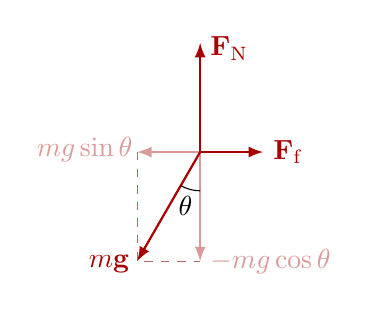
\begin{tikzpicture}
  \def\ang{30} % ground angle
  \def\F{1.6}  % force size
  \def\R{0.18} % ball radius
  \coordinate (O) at (0,0);
  \coordinate (F) at (-90-\ang:\F);
  \coordinate (Fy) at (-90:{\F*cos(\ang)});
  \coordinate (Fx) at (180:{\F*sin(\ang)});
  \draw[dashed,myred!80!black!60] (Fx) -- (F) -- (Fy);
  \draw[Fproj] (O) -- (Fy) node[right=0] {$-mg\cos\theta$}; %\vu{x}
  \draw[Fproj] (O) -- (Fx) node[above=1,left=-2] {$mg\sin\theta$}; %\vu{y}
  \draw[force] (O) -- (F) node[below=1,left=-1] {$m\vb{g}$};
  \draw[force] (O) --++ (90:{\F*cos(\ang)}) node[below=2,right=0] {$\vbF_\mathrm{N}$};
  \draw[force] (O) --++ (0:{\F*sin(\ang)}) node[right=0] {$\vbF_\mathrm{f}$};
  \draw pic["$\theta$",draw=black,angle radius=14,angle eccentricity=1.45] {angle=F--O--Fy};
\end{tikzpicture}


% FRICTION static/dynamical
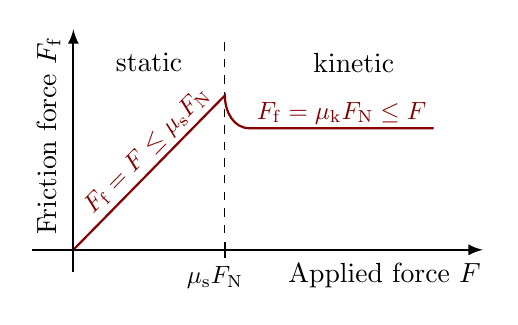
\begin{tikzpicture}
  \def\xmax{5.2}
  \def\ymax{2.8}
  \def\xc{0.37*\xmax}
  \def\yc{0.7*\ymax}
  \draw[dashed] (\xc,0) --++ (0,0.97*\ymax); % coordinate (C);
  \draw[myred!80!black,thick]
    (0,0) -- (\xc,\yc)
    node[scale=0.9,midway,right=5,above=3,rotate={atan2(\yc,\xc)}] {$F_\mathrm{f} = F \leq \mu_\mathrm{s}F_\mathrm{N}$}
    to[out=-90,in=180]++ (0.06*\xmax,-0.08*\xmax) --++ (0.45*\xmax,0)
    node[scale=0.9,midway,above=-2] {$F_\mathrm{f} = \mu_\mathrm{k}F_\mathrm{N} \leq F$};
  \draw[->,thick] (-0.1*\xmax,0) -- (\xmax,0) node[right=4,below left=1] {Applied force $F$};
  \draw[->,thick] (0,-0.1*\ymax) -- (0,\ymax) node[above left=1,rotate=90] {Friction force $F_\mathrm{f}$};
  \draw[thick] (\xc,0.1) --++ (0,-0.2) node[scale=0.9,left=4,below] {$\mu_\mathrm{s}F_\mathrm{N}$};
  \node[] at (\xc/2,0.85*\ymax) {static};
  \node[] at ({(\xmax+\xc)/2},0.85*\ymax) {kinetic};
  
\end{tikzpicture}


\end{document}